\documentclass[12pt,a4paper]{article}
% for Chinese
\usepackage{fontspec}  % 加這個就可以設定字體
\usepackage[BoldFont, SlantFont]{xeCJK}  % 讓中英文字體分開設置
\setCJKmainfont{新細明體}  % 設定中文為系統上的字型,而英文不去更動,使用原TeX\字型

\usepackage{fancyhdr}
\usepackage{graphicx}
\usepackage{geometry}
\usepackage{tabularx}
\usepackage{afterpage}
\usepackage[labelformat=empty]{caption}
\usepackage{titlesec}
\usepackage{hyperref}
\usepackage{enumitem}
\usepackage{lastpage}
\usepackage{textcomp}
\newfontfamily\linesans[Path=Font.assets/]{LINESeedSans_XBd}

\geometry{
a4paper,
left=2cm, right=2cm, top=1.5cm
}
\usepackage{tikz}
\usepackage{amsmath}
\usepackage{lipsum} % for dummy text
\pagestyle{myheadings}
\pagestyle{fancy}
\fancyhf{}

\usepackage{listings}
\usepackage{xcolor}

\definecolor{codegreen}{rgb}{0,0.6,0}
\definecolor{codegray}{rgb}{0.5,0.5,0.5}
\definecolor{codepurple}{rgb}{0.58,0,0.82}
\definecolor{backcolour}{rgb}{0.95,0.95,0.92}

\lstdefinestyle{mystyle}{
    backgroundcolor=\color{backcolour},   
    commentstyle=\color{codegreen},
    keywordstyle=\color{magenta},
    numberstyle=\tiny\color{codegray},
    stringstyle=\color{codepurple},
    basicstyle=\ttfamily\footnotesize,
    breakatwhitespace=false,         
    breaklines=true,                 
    captionpos=b,                    
    keepspaces=true,                 
    numbers=left,                    
    numbersep=5pt,                  
    showspaces=false,                
    showstringspaces=false,
    showtabs=false,                  
    tabsize=2
}

\lstset{style=mystyle}

\newcommand*{\blankpage}{%
\newpage
\vspace*{\fill}
{\centering \huge This page is intentionally left blank.\par}
\vspace{\fill}
\newpage}
\makeatletter
\renewcommand*{\cleardoublepage}{\clearpage\if@twoside \ifodd\c@page\else
\blankpage
\thispagestyle{empty}
\newpage
\if@twocolumn\hbox{}\newpage\fi\fi\fi}
\makeatother

\setlength{\headheight}{40pt}

\renewcommand{\headrulewidth}{1pt}
\renewcommand{\footrulewidth}{2pt}

\fancyhead[C]{\fontsize {10}{12} Programming Design and Optimization 2025

\fontsize{8}{10} Information Management, National Taiwan University, Saturday, April 19th, 2025}

\fancyfoot[C]{Page \thepage \ of \pageref{LastPage}}

\begin{document}
\title{\textbf{NTUIM PDAO 2025}\\ April 19}
\date{}
\maketitle
\thispagestyle{fancy}
\section*{DO NOT turn to next page unless instructed to do so}
\subsection*{CONTEST OVERVIEW}
\begin{itemize} 
    \item The contest runs from 12:00 to 17:00.
    \item There are 14 problems in total, not ordered from easiest to hardest. However, the problems are equally weighted regardless of difficulty.
    \item Teams are ranked according to the most problems solved. Teams who solve the same number of problems are ranked by least total time. The total time is the sum of the time consumed for each problem solved. 
    \item The time consumed for a solved problem is the time elapsed from the beginning of the contest to the submission of the first accepted run plus 20 penalty minutes times the number of any other submission to that problem regardless of submission time. There is no time consumed for a problem that is not solved. If two teams have the same number of problems solved and least total time, then the winner goes to the team who made their first accepted submission on their lastly solved problem earlier.
    \item Each team can only use a single computer with at most one mouse, one screen and one keyboard, so your team members cannot code simultaneously. Allocate your time wisely! 
    \item \textbf{Online Judge}: You have to login to \textbf{PDOGS} with the username and password provided via email to make submissions.
    \item Communicating with any creature other than your teammates is strictly forbidden. Violating this rule may result in a disqualification.
    \item If you have any questions, request a clarification via the Google form in \textbf{PDOGS info}. The judges (i.e. some members in the PDAO Team) will clarify with either \textquotedblleft Yes\textquotedblright, \textquotedblleft No\textquotedblright, \textquotedblleft No Comment\textquotedblright\ or \textquotedblleft Pardon\textquotedblright.
\end{itemize}

\noindent\vfill
\begin{minipage}{0.97\textwidth}
 \noindent\hfill PDAO 2025 is sponsored by \textcopyright \space {\linesans LINE}
\end{minipage}

\blankpage

\section*{\fontsize{18}{12}Problem A. Mischievous Elves and Magic Sorting Spell}

\begin{alignat*} {2}
 &   \text{Input file:}   \quad     &&\text{stdin}\\
 &   \text{Output file:}  \quad     &&\text{stdout}\\
 &   \text{Time limit:}   \quad     &&\text{1 second}\\
 &   \text{Memory limit:} \quad     &&\text{64 MB}
\end{alignat*}
\noindent
Deep in an enchanted forest, a group of mischievous elves loves playing a game called \textbf{Number Gathering}. During the game, they arrange a row of magic stones, each with a value in a completely random order!
\\\\
\noindent
The Elf King, however, has established a \textbf{sacred rule} for how these number stones should be arranged:

\begin{itemize}
    \item One of the \textbf{largest} valued stones must be placed in the \textbf{rightmost} position.
    \item One of the \textbf{smallest} valued stones must be placed in the \textbf{leftmost} position.
\end{itemize}

\noindent
The elves possess a special power -- the \textbf{Adjacent Swap Spell}, which allows them to swap two neighboring stones. Now, the Elf King wants to know:
\\\\
\noindent
What is the \textbf{minimum number of swaps} needed to rearrange the stones to satisfy his rule?

\subsection*{\fontsize{16}{12}Input}
Line 1 contains a single integer $N$, denoting the quantity of stones. \\\\
Line 2 contains $N$ integers $v_i$, denoting the number of each stone. 

\begin{itemize}
    \item $1 \leq N \leq 100000$
    \item $1 \leq v_i \leq 100000$
\end{itemize}

\subsection*{\fontsize{16}{12}Output}
Print a single integer, the minimum number of adjacent swaps required to place:
\begin{itemize}
    \item One of the smallest valued stones at the leftmost position.
    \item One of the largest valued stones at the rightmost position.
\end{itemize}

\newpage
\subsection*{\fontsize{16}{12}Example}
\begin{table}[h]
  \centering
  \begin{tabularx}{\textwidth}{|>{\ttfamily}X|>{\ttfamily}X|}
  \hline
  stdin & stdout \\
  \hline
    6 & 3 \\
    3 4 1 5 5 3 & \\
  \hline
  \end{tabularx}
\end{table}

\subsection*{\fontsize{16}{12}Explanation}
Given the initial arrangement: \{3, 4, 1, 5, 5, 3\}

\begin{enumerate}
    \item Swap index 1 and 2: \{3, \underline{1}, \underline{4}, 5, 5, 3\}
    \item Swap index 0 and 1: \{\underline{1}, \underline{3}, 4, 5, 5, 3\} (smallest valued is now at the leftmost position)
    \item Swap index 4 and 5: \{1, 3, 4, 5, \underline{3}, \underline{5}\} (largest valued is now at the rightmost position)
\end{enumerate}
Thus, the minimum number of swaps required is \textbf{3}.
\newpage
\section*{\fontsize{18}{12}Problem B. Stock Price Prediction Adjustment}

\begin{alignat*} {2}
 &   \text{Input file:}   \quad     &&\text{stdin}\\
 &   \text{Output file:}  \quad     &&\text{stdout}\\
 &   \text{Time limit:}   \quad     &&\text{1 second}\\
 &   \text{Memory limit:} \quad     &&\text{64 MB}
\end{alignat*}

\noindent
HappyCorp, a leading investment firm, predicts stock prices daily. However, when compared to actual prices, the prediction error is too high! To save their reputation, they can adjust one prediction by swapping it with another from their forecast. 
\\\\
\noindent
Analysts have access to two sequences of positive integers representing stock prices:

\begin{itemize}
    \item \textbf{predicted prices}: The stock prices predicted over a period of $n$ days.
    \item \textbf{actual prices}: The actual stock prices observed over the same $n-day$ period.
\end{itemize}

\noindent 
The \textbf{total prediction error} is defined as the sum:

\[
\sum_{i=0}^{n-1} \left| \textbf{actual prices}_i - \textbf{predicted prices}_i \right|
\]

\noindent You are allowed to replace \textbf{at most one} element of \textbf{predicted prices} with \textbf{any} other element in \textbf{predicted prices} to \textbf{minimize} the total prediction error. 
\\\\
\noindent
Your task is to determine the \textbf{minimum possible total prediction error} after making at most one such replacement.

\subsection*{\fontsize{16}{12}Input}
Line 1 contains a single integer $N$, denoting the number of days. \\\\
Line 2 contains $N$ positive integers $p_i$, denoting the \textbf{predicted stock prices}. \\\\
Line 3 contains $N$ positive integers $a_i$, denoting the \textbf{actual stock prices}.
\\\\
\noindent Constraints:
\begin{itemize}
    \item \( 1 \leq N \leq 10^5 \)
    \item \( 1 \leq p_i, a_i \leq 10^5\quad\forall i \in [0, N)\)
\end{itemize}

\subsection*{\fontsize{16}{12}Output}
Print a single integer, the minimum possible total prediction error after at most one replacement.

\subsection*{\fontsize{16}{12}Example}
\begin{table}[h]
  \centering
  \begin{tabularx}{\textwidth}{|>{\ttfamily}X|>{\ttfamily}X|}
  \hline
  stdin & stdout \\
  \hline
    3 & 3 \\
    1 7 5 & \\
    2 3 5 & \\  
  \hline
  \end{tabularx}
\end{table}

\subsection*{\fontsize{16}{12}Explanation}
Given:
\[
\textbf{predicted prices} = [1, 7, 5], \quad \textbf{actual prices} = [2, 3, 5]
\]
The initial absolute sum difference is:
\[
\left| 1 - 2 \right| + \left| 7 - 3 \right| + \left| 5 - 5 \right| = 1 + 4 + 0 = 5.
\]

\noindent The optimal solution is:
\begin{itemize}
    \item Replace the second element ($7$) with the first element ($1$), yielding:
    \[
    [1, \mathbf{1}, 5]
    \]
    The new sum difference is:
    \[
    \left| 1 - 2 \right| + \left| 1 - 3 \right| + \left| 5 - 5 \right| = 1 + 2 + 0 = 3.
    \]
    
    \item Alternatively, replace the second element ($7$) with the third element ($5$), yielding:
    \[
    [1, \mathbf{5}, 5]
    \]
    The new sum difference is:
    \[
    \left| 1 - 2 \right| + \left| 5 - 3 \right| + \left| 5 - 5 \right| = 1 + 2 + 0 = 3.
    \]
\end{itemize}

\noindent Since both cases yield a minimum absolute sum difference of \( 3 \), the output is: $3$
\newpage

\section*{\fontsize{18}{12}Problem C. Xiangqi }

\begin{alignat*} {2}
 &   \text{Input file:}   \quad     &&\text{stdin}\\
 &   \text{Output file:}  \quad     &&\text{stdout}\\
 &   \text{Time limit:}   \quad     &&\text{1 second}\\
 &   \text{Memory limit:} \quad     &&\text{64 MB}
\end{alignat*}
\noindent
Two Xiangqi masters Tokugawa and Gashuin said they've beaten every other master in the world. However, some said that there
are some players with sharper skills. This brought them here
to challenge master Junpi and Mahiro. There will be an award if they win or be a punishment.
Therefore, they're careful about their play and clench every chance to win.
\\\\
\noindent
Now let\textquotesingle s introduce the rules of Xiangqi:
\\\noindent
Xiangqi is a game represents a battle between two armies with the goal
of capturing the enemy's \textbf{general} piece. In this problem, you are
given a situation of later stages in the game, you need to check
whether you've already win after your move, i.e. you can't be \textbf{checkmated} while black has \textbf{no available moves} to prevent themself from being \textbf{checked} or \textbf{stalemate}.
\\\\
\noindent
Xiangqi is played on a $10\times9$ board and pieces are
placed on the points. The upper left point is (1,1) and
the lower right point is (10,9). There are two groups of pieces marked
by black or red Chinese characters, belonging to the two players
separately.
\\\\
\noindent
Each player, in turn, moves one piece from its own point to another point. No two pieces can occupy the
same point at the same time. A piece can be moved to a point occupied
by an enemy piece, in which case the enemy piece is \textbf{captured} and
removed from the board. 
\\\\
\noindent
When the \textbf{general} is in danger of captured
by the enemy player on the enemy player's next move, the enemy player is
said to have \textbf{delivered a check}. If the general's player can make no
move to prevent the general's capture by next enemy move, the situation called \textbf{checkmate}.
\\\\
\noindent
Each piece\textquotesingle s introduction is as follows:
\\\noindent
\textbf{\includegraphics{Xiangqi.assets/75px-Xiangqi_General.png}General:}
the generals can move and capture one point either vertically or
horizontally and cannot leave the \textbf{palace} unless the situation called
\textbf{flying general}. \textbf{Flying general} means that
one general can \textbf{fly} across the board to capture the enemy general if
they stand on the same line without intervening pieces.
\\\noindent
\textbf{\includegraphics{Xiangqi.assets/75px-Xiangqi_Advisor.png}Advisor:}
the advisors can move and capture one point diagonally and may not leave
the palace, which confines them to five points on the board.
\\\noindent
\textbf{\includegraphics{Xiangqi.assets/75px-Xiangqi_Elephant.png}Elephant:}
the elephants move and capture exactly two points diagonally and may not
jump over the intervening pieces; the move like the
character \textbf{田}, in reference to the board\textquotesingle s squares. 
However, it is possible to block an elephant with a diagonally adjacent piece, known as \textbf{blocking
elephant\textquotesingle s eye} (see the figure below). When this
happens, it cannot move or capture in that direction. The elephant cannot cross the river.
\\\noindent
\textbf{\includegraphics{Xiangqi.assets/75px-Xiangqi_Chariot.png}Chariot:}
the chariots can move and capture vertically and horizontally by any
distance, but may not jump over the intervening pieces.
\\\noindent
\textbf{\includegraphics{Xiangqi.assets/75px-Xiangqi_Cannon.png}Cannon:}
the cannons move like the chariots, horizontally and vertically, but
capture by jumping exactly one piece (whether it is friendly or enemy)
over to its target.
\\\noindent
\textbf{\includegraphics{Xiangqi.assets/75px-Xiangqi_Horse.png}Horse:}
the horses have 8 kinds of jumps to move and capture shown in the left
figure. However, if there is any pieces lying on a point away from the
horse horizontally or vertically it cannot move or capture in that
direction (see the figure below), called \textbf{hobbling horse's
leg}. Now you are given a situation only containing a black general, a
red general and several red chariots, cannons and horses, and the red
side has delivered a check. Now it turns to black side's move. Your job
is to determine that whether this situation is \textbf{checkmate}.
\\\noindent
\textbf{\includegraphics{Xiangqi.assets/75px-Xiangqi_Soldier.png}Soldier:}
the solders move and capture by advancing one point. Once they have
crossed the river, they may also move and capture one point
horizontally. Soldiers cannot move backward, and therefore cannot
retreat; after advancing to the last rank of the board, however, a
soldier may still move sideways at the enemy\textquotesingle s edge.
\begin{figure}[htbp]
    \centering
    \begin{minipage}[b]{0.3\textwidth}
        \centering
        \includegraphics[width=\linewidth]{Xiangqi.assets/Board.jpg}
        \caption{Game Board}
    \end{minipage}
    \begin{minipage}[b]{0.25\textwidth}
        \centering
        \includegraphics[width=\linewidth]{Xiangqi.assets/180px-MovementOfHorsePiece.png}
        \caption{hobbling horse's leg}
    \end{minipage}
    \begin{minipage}[b]{0.27\textwidth}
        \centering
        \includegraphics[width=\linewidth]{Xiangqi.assets/Elephant_movement.png}
        \caption{blocking elephant\textquotesingle s eye}
    \end{minipage}
\end{figure}
\\
\noindent
Please be noted that only the soldier, horse, canon and chariot can cross the river.
\\
\noindent
Now give you a table of later game, you need to check if you have already won the game. It's not necessary mean checkmate (Stalemate also indicates a win in Xiangqi).
\textbf{You always play red} (i.e., the one on the bottom). You have already made your move while the other hasn't.
\subsection*{\fontsize{16}{12}Input}
Given a $10\times9$ array full of characters, where the general, advisor, elephant, chariot, horse, canon, soldier, and empty space are represented by G, S, E, R, H, C, P, and . (a single dot) respectively. Upper cases indicate Black player while lower cases indicate red player.
\subsection*{\fontsize{16}{12}Output}
A single line of "Yes" or "No", indicating if you(\textbf{Red player}) have already won the game.
\subsection*{\fontsize{16}{12}Examples}
\begin{table}[h]
  \centering
  \begin{tabularx}{\textwidth}{|>{\ttfamily}X|>{\ttfamily}X|}
  \hline
  stdin & stdout\\
  \hline
    ...G.....&No\\
    ..r......&\\
    .........&\\
    .........&\\
    .........&\\
    .........&\\
    .......P.&\\
    .........&\\
    .........&\\
    ....g....&\\
  \hline
 \end{tabularx}
\end{table}

\begin{table}[h]
  \centering
  \begin{tabularx}{\textwidth}{|>{\ttfamily}X|>{\ttfamily}X|}
  \hline
  stdin & stdout\\
  \hline
    ...G.....&Yes\\
    ..r......&\\
    .........&\\
    .........&\\
    .........&\\
    .........&\\
    .........&\\
    .........&\\
    .........&\\
    ....g....&\\
  \hline
 \end{tabularx}
\end{table}

\subsection*{\fontsize{16}{12}Explanation}
Notice that in Sample 1 and Sample 2, both of the black generals are unable to move since all of the spaces near them are being attacked. However, one plays the black has one pawn in Sample 1. Therefore, they are able to move the pawn and the game shall go on. Not like in Sample 2 where they don't have any choice other than move their general, which leads to their general being capture by their opponent.


\subsection*{\fontsize{16}{12}Notes}
\begin{itemize}
\item  The situation presented will always be achievable in normal game play, and you have already made your move while your opponent hasn't.
\item Only the soldier, horse, canon and chariot can
cross the river.
\item You cannot be checked.
\end{itemize}

\blankpage

\section*{\fontsize{18}{12}Problem D. Pirate Code: The Black Spot Game}

\begin{alignat*} {2}
 &   \text{Input file:}   \quad     &&\text{stdin}\\
 &   \text{Output file:}  \quad     &&\text{stdout}\\
 &   \text{Time limit:}   \quad     &&\text{100 milliseconds}\\
 &   \text{Memory limit:} \quad     &&\text{64 MB}
\end{alignat*}
\noindent
During the Golden Age of Piracy, Captain Henry Ironhook Vance and his crew of \(N\) pirates had just seized the legendary Bloodstone Compass-a mystical artifact said to guide its owner to untold riches. 
But greed is a pirate's curse, and the crew soon fell into a deadly dispute over who would claim it.\\
\noindent\\
Following the ancient Pirate Code, they resorted to the dreaded Black Spot Game to decide. 
%Here, we will first introduce the famous Black Spot Game: forming a circle, the \(M\) pirates passed around the cursed medallion. 
%Every \(K^{th}\) pirate to receive the medallion was marked for doom and thrown overboard. 
In this infamous game, the $M$ pirates formed a circle and passed around the cursed medallion. Every $K^{th}$ pirate to receive the medallion was marked for doom and thrown overboard.
The process repeated until only one pirate remained.\\
\noindent\\
Here is a detailed description of the Black Spot Game:
Before the game starts, there will be \(m\) pirates in total and an elimination number \(k\) will be pre-decided.
\begin{enumerate}
    \setlength{\itemsep}{-3pt} % Reduce space between items
    \item A total of \(M\) pirates (numbered 0 to \(M-1\)) stand in a circle.
    \item The game starts at pirate 0.
    \item Counting proceeds \textbf{clockwise}, eliminating every \(K^{th}\) pirate.
    \item The pirate who is eliminated is \textbf{removed} from the circle.
    \item The next round starts with the pirate immediately clockwise to the eliminated one.
    \item The process continues until only one pirate remains.
\end{enumerate}

\noindent
For a more detailed illustration of how Black Spot Game proceeds, below is an illustration of the 
Black Spot Game with a total of \(M = 5\) pirates and elimination number \(K = 2\).
\begin{center}
    \begin{tikzpicture}[scale=0.9]
        
        \begin{scope}[shift={(-6.25,0)}] 
            % Draw eliminated pirate
            \node[circle, draw, fill=white!50, minimum size=1.2cm] (2) at (18:2.5cm) {\textbf{2}};
        \end{scope}

        % First Circle (Initial State)
        \begin{scope}[shift={(-6.25,0)}] % Adjust position for first diagram
            % Draw large outer circle
            \draw[thick] (0,0) circle (2.5cm);
        
            % Draw remaining pirates (white)
            \foreach \i/\label in {90/0, -54/2, -126/3, 162/4} {
                \node[circle, draw, fill=white!50, minimum size=1cm] (\label) at (\i:2.5cm) {\textbf{\label}};
            }
            % Draw eliminated pirate
            \node[circle, draw, fill=white!50, minimum size=1cm] (2) at (18:2.5cm) {\textbf{1}};

            % Label step number
            \node at (-3, 2.5) {\textbf{1)}};
        \end{scope}

        % Second Circle (After eliminating 1)
        \begin{scope}[shift={(0,0)}]
            % Draw eliminated pirate (red)
            \node[circle, draw, fill=white!50, minimum size=1.2cm] (4) at (-126:2.5cm) {\textbf{4}};
        \end{scope}
        
        % Second Circle (After eliminating 1)
        \begin{scope}[shift={(0,0)}] % Adjust position for second diagram
            % Draw large outer circle
            \draw[thick] (0,0) circle (2.5cm);
        
            % Draw remaining pirates
            \foreach \i/\label in {90/0, -54/2, 162/4} {
                \node[circle, draw, fill=white!50, minimum size=1cm] (\label) at (\i:2.5cm) {\textbf{\label}};
            }
            % Draw eliminated pirate
            \node[circle, draw, fill=white!50, minimum size=1cm] (4) at (-126:2.5cm) {\textbf{3}};
            
            % Label step number
            \node at (-3, 2.5) {\textbf{2)}};
        \end{scope}

        % Third Circle (After eliminating 3)
        \begin{scope}[shift={(6,0)}]
            % Draw eliminated pirate (red)
            \node[circle, draw, fill=white!50, minimum size=1.2cm] (1) at (90:2.5cm) {\textbf{1}};
        \end{scope}

        % Third Circle (After eliminating 3)
        \begin{scope}[shift={(6,0)}] % Adjust position for third diagram
            % Draw large outer circle
            \draw[thick] (0,0) circle (2.5cm);
        
            % Draw remaining pirates
            \foreach \i/\label in {-54/2, 162/4} {
                \node[circle, draw, fill=white!50, minimum size=1cm] (\label) at (\i:2.5cm) {\textbf{\label}};
            }
            % Draw eliminated pirate
            \node[circle, draw, fill=white!50, minimum size=1cm] (1) at (90:2.5cm) {\textbf{0}};

            % Label step number
            \node at (-3, 2.5) {\textbf{3)}};
        \end{scope}
    \end{tikzpicture}
    \newpage
    \begin{tikzpicture}[scale=0.9] % Adjust scale to fit better

        % Fourth Circle (After eliminating 0)
        \begin{scope}[shift={(-3,-4)}] 
            % Draw eliminated pirate (red)
            \node[circle, draw, fill=white!50, minimum size=1.2cm] (4) at (162:2.5cm) {\textbf{4}};
        \end{scope}
        
        % Fourth Circle (After eliminating 0)
        \begin{scope}[shift={(-3,-4)}] % Position fourth diagram
            % Draw large outer circle
            \draw[thick] (0,0) circle (2.5cm);
        
            % Draw remaining pirate
            \node[circle, draw, fill=white!50, minimum size=1cm] (2) at (-54:2.5cm) {\textbf{2}};
            
            % Draw eliminated pirate (red)
            \node[circle, draw, fill=white!50, minimum size=1cm] (4) at (162:2.5cm) {\textbf{4}};

            % Label step number
            \node at (-3, 2.3) {\textbf{4)}};
        \end{scope}

        % Fifth Circle (Final Winner)
        \begin{scope}[shift={(3,-4)}] % Position fifth diagram
            % Draw large outer circle
            \draw[thick] (0,0) circle (2.5cm);
        
            % Draw winner pirate (green)
            \node[circle, draw, fill=white!50, minimum size=1cm] (2) at (-54:2.5cm) {\textbf{2}};

            % Label step number
            \node at (-2.5, 2.3) {\textbf{5)}};
        \end{scope}
    \end{tikzpicture}
\end{center}

\noindent
Each pirate is labeled with a number from 0 to 4 in clockwise direction. Each round, one pirate will be eliminated. 
The eliminated pirate is labeled in a double-circle. The winner is the last remaining pirate, which is pirate number 2.\\

\noindent
However, after listening to the explanation of the game, the pirates thought that it was too plain and simple.
To make the game more complex and sophisticated, the pirates decide to elevate the game to another level. The \(P\) pirates will be divided into \(N\) \textbf{non-identical groups}, 
each group \(i \in \{0, 1, ..., N-1\}\) will consist of \(M_i\) pirates, and the group will be assigned an elimination number \(K_i\).
\textbf{Every group will play the Black Spot Game until only one pirate remain in the group.} After all groups have sort out a final survivor,
the \(N\) remaining pirates (one from each group) will gather to \textbf{play one final round} of the Black Spot Game, their numbers in the last round are their own group number, and the final round will be assigned an elimination number \(K_f\).The last pirate to survive this round will be the true heir to the untold treasures.\\

\noindent
Your task is to determine which pirate will outlast the curse and claim their fortune.
You will need to determine which group the winning pirate was originally in, and the pirate's number in that original group. 

\subsection*{\fontsize{16}{12}Input}
The first line of input consists of two integers \(N\) and \(K_f\):\\
\begin{itemize}
    \item \(1 \leq N \leq 500\) Representing the number of groups to split the pirates in,
    \item \(1 \leq K_f \leq N\) Denoting the elimination number for the \textbf{final round}.
\end{itemize}
The following \(N\) lines will each represent every group of pirates, each line consist of two integers \(M_i\) and \(K_i\), \(i\) denotes the group number.\\
\indent
\begin{itemize}
    \item \(1 \leq M_i \leq 500\) Denoting the number of pirates in group \(i\),
    \item \(1 \leq K_i \leq M_i\) Denoting the assigned elimination number for group \(i\).
\end{itemize}
\noindent
Note that we did not explicitely input the total number of pirates onboard \(P\), since 
\(\Sigma_{i=0}^{N-1}M_i=P\) (number of pirates in each group will naturally sum up to \(P\)).\\

\noindent
Please also note that the groups are non-identical, so the number of pirates in each group varies, 
the elimination number for each group also varies.\\


\subsection*{\fontsize{16}{12}Output}
You should output two integers to tell us who the winner is:\\
\indent
1. The group the winner was initially in.\\
\indent
2. The number of the winner in the group.\\

\noindent
For example, the winner was in the group $0$, and was the number $2$ pirate in the group, output 0 2. 
\subsection*{\fontsize{16}{12}Example 1}
% Example Table
\begin{table}[h]
    \centering
    \begin{tabularx}{\textwidth}{|>{\ttfamily}X|>{\ttfamily}X|}
    \hline
    \textbf{stdin} & \textbf{stdout} \\
    \hline
    5 2 & 2 3 \\
    6 3 & \\
    7 4 & \\
    10 3 & \\
    3 2 & \\
    5 2 & \\
    \hline
    \end{tabularx}
\end{table}

\subsection*{\fontsize{16}{12}Example 2}
% Example Table
\begin{table}[h]
    \centering
    \begin{tabularx}{\textwidth}{|>{\ttfamily}X|>{\ttfamily}X|}
    \hline
    \textbf{stdin} & \textbf{stdout} \\
    \hline
    7 3 & 3 2 \\
    10 2 & \\
    5 3 & \\
    4 3 & \\
    5 2 & \\
    12 4 & \\
    21 10 & \\
    8 3 & \\
    \hline
    \end{tabularx}
\end{table}

\blankpage

\section*{\fontsize{18}{12}Problem E. The Museum's Security Grid}

\begin{alignat*} {2}
 &   \text{Input file:}   \quad     &&\text{stdin}\\
 &   \text{Output file:}  \quad     &&\text{stdout}\\
 &   \text{Time limit:}   \quad     &&\text{500 milliseconds}\\
 &   \text{Memory limit:} \quad     &&\text{64 MB}
\end{alignat*}

\noindent
The prestigious National Museum of Technology operates a high-tech security system based on an \(M \times N\) grid of laser sensors. Each sensor has a \textbf{unique} power level used to detect intruders. However, the chief security officer noticed that the power levels are unnecessarily high, leading to excessive energy consumption.
\\\\
\noindent
To optimize energy efficiency, the power levels must be reconfigured while preserving the system's effectiveness. The new configuration must satisfy the following conditions:
\begin{itemize}
    \item If a sensor originally had a higher power level than another sensor in the \textbf{same row or column}, it must remain more powerful in the new configuration.
    \item The highest power level in the new configuration must be \textbf{as low as possible}.
    \item The minimum power level in the new configuration must be \textbf{at least 1}.
\end{itemize}

\noindent
As the museum's security consultant, your task is to determine the optimal power levels for each sensor in the grid while ensuring that the conditions above are met.

\subsection*{\fontsize{16}{12}Input}
Line 1 contains two integers \(M\) and \(N\), denoting the number of rows and columns in security grid.
\\\\
\noindent
The next \(M\) lines each contain \(N\) integers, denoting the number of the sensors in the grid and $P$ denoting the power levels of the sensors. Each power level in initial configuration is \textbf{unique}.
\begin{itemize}
    \item \(1 \leq M, N \leq 1000\)
    \item $1\leq P \leq 10^5$
    \item $P \text{ is unique}$
    \item \(M \cdot N \leq 10^5\)
\end{itemize}
\subsection*{\fontsize{16}{12}Output}
Output \(M\) lines, each containing \(N\) space-separated integers, denoting the reconfigured security grid.

\subsection*{\fontsize{16}{12}Example 1}
\begin{table}[h]
  \centering
  \begin{tabularx}{\textwidth}{|>{\ttfamily}X|>{\ttfamily}X|}
  \hline
  \textbf{stdin} & \textbf{stdout} \\
  \hline
  2 2 & 2 1 \\
  3 1 & 1 2 \\
  2 5 & \\
  \hline
  \end{tabularx}
\end{table}

\subsection*{\fontsize{16}{12}Explanation}
The original grid is:

\[
\begin{bmatrix}
3 & 1 \\
2 & 5
\end{bmatrix}
\]
\noindent
After reconfiguration, the new grid is:

\[
\begin{bmatrix}
2 & 1 \\
1 & 2
\end{bmatrix}
\]

\noindent The maximum power level in this new grid is 5, and it can be shown that no smaller power level configuration satisfies the conditions.

\subsection*{\fontsize{16}{12}Example 2}
\begin{table}[h]
  \centering
  \begin{tabularx}{\textwidth}{|>{\ttfamily}X|>{\ttfamily}X|}
  \hline
  \textbf{stdin} & \textbf{stdout} \\
  \hline
  1 1 & 1 \\
  10 & \\
  \hline
  \end{tabularx}
\end{table}

\subsection*{\fontsize{16}{12}Explanation}
Since there is only one sensor, it must be assigned the minimum power level of 1.

\newpage

\section*{\fontsize{18}{12}Problem F. The Ancient Formula}

\begin{alignat*} {2}
 &   \text{Input file:}   \quad     &&\text{stdin}\\
 &   \text{Output file:}  \quad     &&\text{stdout}\\
 &   \text{Time limit:}   \quad     &&\text{1 second}\\
 &   \text{Memory limit:} \quad     &&\text{64 MB}
\end{alignat*}
\noindent
During an archaeological dig, Dr. Yee discovered a collection of ancient tablets containing strange chemical formulas written in an old script. After careful translation by his research team, the formulas were finally decoded.
\\\\
\noindent
As a modern chemist, Dr. Yee recognized some of the symbols as elements, but the structure seemed unusual. Was this an early attempt at chemical notation, or could it represent something valuable?
\\\\
\noindent
Upon further investigation, Dr. Yee noticed that some of the formulas resembled those in his notes. However, the ancient formulas used parentheses and had different groupings, raising an important question: Were they describe the same compound, but in a different notation system?
\\\\
\noindent
Can you help Dr. Yee verify whether the ancient formula matches the modern one?

\subsection*{\fontsize{16}{12}Input}
Line 1 contains two integers $N_1$ and $N_2$, denoting the length of following two formulas.
\\\\
\noindent
Line 2 - 3 each contains a string represents ancient and modern formula respectively.\\\\
\noindent
A formula follows these rules:  
\begin{itemize}
    \item An atom is denoted as a uppercase letter and may followed by a lowercase letter. 
    \item An element can be a group of atoms, elements, or both.
    \item Digits (ranging from 1 to 100) following an atom or element indicate the quantity. If no digit is present, the quantity is assumed to be 1.  
    \item Parentheses are used to group elements and can be followed by a number, indicating how many times the group should be repeated.
    \item Parentheses may be used to group elements, with a maximum nesting depth of \( 15 \).
    \item The number of every atom in each formula will not exceed \(10^5\).
    \item $1 \leq N_1, N_2 \leq 10^4$
\end{itemize}  
\noindent
\textit{Note: The atoms and elements in these formulas may not necessarily exist on Earth, as Dr. Yee lives in a different universe.}  


\subsection*{\fontsize{16}{12}Output}
Two formulas are considered to represent the same compound if they contain exactly the same atoms in identical quantities, regardless of how they are grouped. Therefore, the output will be either "Yes" or "No".

\subsection*{\fontsize{16}{12}Example 1}
\begin{table}[h]
  \centering
  \begin{tabularx}{\textwidth}{|>{\ttfamily}X|>{\ttfamily}X|}
    \hline
    stdin & stdout \\
    \hline
    10 8 & No \\
    (X3(OR)2)3 & \\
    X8(OR2)3 &  \\
    \hline
  \end{tabularx}
\end{table}

\subsection*{\fontsize{16}{12}Explanation}

Expanding the formulas:
\begin{itemize}
    \item \texttt{(X3(OR)2)3} expands as:
      \begin{itemize}
          \item \texttt{X3} is repeated 3 times $\rightarrow$ \texttt{X9}
          \item \texttt{(OR)2} expands to \texttt{O2R2}, and repeating this 3 times gives \texttt{O6R6}.
      \end{itemize}
      So, the full expansion is \texttt{X9O6R6}.
      
    \item \texttt{X8(OR2)3} expands as:
      \begin{itemize}
          \item \texttt{X8} remains as is.
          \item \texttt{(OR2)3} expands to \texttt{O3R6}.
      \end{itemize}
      So, the full expansion is \texttt{X8O3R6}.
\end{itemize}
\noindent
Since the number of atoms does not match, the two formulas represent different compounds.

\subsection*{\fontsize{16}{12}Example 2}
\begin{table}[h]
  \centering
  \begin{tabularx}{\textwidth}{|>{\ttfamily}X|>{\ttfamily}X|}
    \hline
    stdin & stdout \\
    \hline
    9 15 & Yes \\ 
    SO2(ORe)4 & \\
    (ORe)2S(ORe)2O2 & \\
    \hline
  \end{tabularx}
\end{table}

\subsection*{\fontsize{16}{12}Explanation}
Expanding both formulas:
\begin{itemize}
    \item \texttt{SO2(ORe)4} expands to \texttt{S1O6Re4}.
    \item \texttt{(ORe)2S(ORe)2O2} expands to \texttt{S1O6Re4}.
\end{itemize}

Since both formulas contain the same elements in the same quantities, they represent the same compound.

\newpage

\section*{\fontsize{18}{12}Problem G. Magic Potion Battle}

\begin{alignat*} {2}
 &   \text{Input file:}   \quad     &&\text{stdin}\\
 &   \text{Output file:}  \quad     &&\text{stdout}\\
 &   \text{Time limit:}   \quad     &&\text{500 milliseconds}\\
 &   \text{Memory limit:} \quad     &&\text{64 MB}
\end{alignat*}

\noindent
In the dark ages of wizardry, the legendary sorcerers Merlin and Morgana engaged in a fierce \textbf{Magic Potion Battle}. In this battle, they took turns casting spells to destroy potion bottles infused with magical essence. 
\\\\
\noindent
The game follows these rules:
\begin{itemize}
    \item Merlin and Morgana take turns destroying exactly one potion bottle per turn.
    \item Merlin always plays first.
    \item The game ends immediately if the total amount of magical essence destroyed becomes \textbf{divisible by 3}. The player who made that move \textbf{loses}.
    \item If all potions are destroyed and the total essence is \textbf{not} divisible by 3, \textbf{Morgana automatically wins}.
\end{itemize}

\noindent
Both players play \textbf{optimally}, meaning they make the best possible moves to maximize their chances of winning. 
\\\\
\noindent
Your task is to determine whether Merlin can guarantee a win, or if Morgana will inevitably win. Print `"Yes"` if Merlin wins and `"No"` if Morgana wins.

\subsection*{\fontsize{16}{12}Input}
Line 1 contains a single integer \( N \) \((1 \leq N \leq 10^5)\), representing the number of potion bottles.
\\\\
\noindent
Line 2 contains \( N \) space-separated integers, where the \( i^{th} \) integer represents the magical essence in the \( i^{th} \) potion bottle. Each integer \( K \) satisfies \( 1 \leq K \leq 10^4 \).

\subsection*{\fontsize{16}{12}Output}
Print "Yes" if Merlin can force a win; otherwise, print "No".

\subsection*{\fontsize{16}{12}Example 1}
\begin{table}[h]
  \centering
  \begin{tabularx}{\textwidth}{|>{\ttfamily}X|>{\ttfamily}X|}
  \hline
  \textbf{stdin} & \textbf{stdout} \\
  \hline
  2 & Yes \\
  2 1 & \\
  \hline
  \end{tabularx}
\end{table}

\subsection*{\fontsize{16}{12}Explanation}
The game proceeds as follows:
\begin{itemize}
    \item \textbf{Turn 1:} Merlin removes either potion bottle.
    \item \textbf{Turn 2:} Morgana removes the remaining bottle. 
\end{itemize}
The sum of the destroyed potion bottles is \( 2 + 1 = 3 \), which is divisible by 3. Since Morgana made the move that resulted in this, she \textbf{loses}, and Merlin wins.

\subsection*{\fontsize{16}{12}Example 2}
\begin{table}[h]
  \centering
  \begin{tabularx}{\textwidth}{|>{\ttfamily}X|>{\ttfamily}X|}
  \hline
  \textbf{stdin} & \textbf{stdout} \\
  \hline
  5 & No \\
  5 1 2 4 3 & \\
  \hline
  \end{tabularx}
\end{table}

\subsection*{\fontsize{16}{12}Explanation}
One possible sequence of moves for Morgana to win:
\begin{itemize}
    \item \textbf{Turn 1:} Merlin removes the potion with value 1. Sum = \( 1 \).
    \item \textbf{Turn 2:} Morgana removes the potion with value 3. Sum = \( 1 + 3 = 4 \).
    \item \textbf{Turn 3:} Merlin removes the potion with value 4. Sum = \( 1 + 3 + 4 = 8 \).
    \item \textbf{Turn 4:} Morgana removes the potion with value 2. Sum = \( 1 + 3 + 4 + 2 = 10 \).
    \item \textbf{Turn 5:} Merlin removes the potion with value 5. Sum = \( 1 + 3 + 4 + 2 + 5 = 15 \).
\end{itemize}
Since 15 is divisible by 3, Merlin \textbf{loses}, meaning Morgana wins. Thus, the output is "No".

\newpage

\section*{\fontsize{18}{12}Problem H. Ingenious Missions}

\begin{alignat*} {2}
 &   \text{Input file:}   \quad     &&\text{stdin}\\
 &   \text{Output file:}  \quad     &&\text{stdout}\\
 &   \text{Time limit:}   \quad     &&\text{1 second}\\
 &   \text{Memory limit:} \quad     &&\text{64 MB}
\end{alignat*}

\noindent
You are the mastermind behind a covert operations unit tasked with executing high-stakes missions. Your team consist of a fixed number of agents and a list of \( m \) planned missions. 
\\\\
\noindent
Your goal is to select a subset of missions to achieve \textbf{at least} a total benefit of \( r \) while using \textbf{at most} \( n \) agents in total.
\\\\
\noindent
There are some requirements for each mission:
\begin{itemize}
  \item Each mission requires a specific number of agents and yields a corresponding benefit.
  \item Each mission can be executed at most once.
  \item Each agent can be assigned to only one mission.
\end{itemize}

\noindent
The order in which missions are selected does not matter; only the set of missions chosen determines the outcome.

\subsection*{\fontsize{16}{12}Input}
Line 1 contains three integers \( N \), \( R \), \( M \), denoting the \textbf{number of agents available}, the \textbf{minimum required benefit}, and the \textbf{number of missions}, respectively.
\\\\
The next \( M \) lines each contain two integers \( G_i \) and \( B_i \), denoting the \textbf{agents required to execute the mission}, the \textbf{benefit received from the mission}, respectively.
\begin{itemize}
    \item \(1 \leq N,R,M \leq 100\)
    \item \(1 \leq G_i,B_i \leq 100\quad \forall\ i \in [0, M)\)
\end{itemize}

\subsection*{\fontsize{16}{12}Output}
Print a single integer, the total number of valid mission schemes modulo \( 10^9 + 7 \).

\subsection*{\fontsize{16}{12}Example}

\begin{table}[h]
  \centering
  \begin{tabularx}{\textwidth}{|>{\ttfamily}X|>{\ttfamily}X|}
  \hline
  \textbf{stdin} & \textbf{stdout} \\
  \hline
  5 3 3 & 5 \\
  2 2 & \\
  2 3 & \\
  1 1 & \\
  \hline
  \end{tabularx}
\end{table}

\subsection*{\fontsize{16}{12}Explanation}

There are 3 missions:
\begin{itemize}
 \item \textbf{Mission 0}: Requires 2 agents($G_0$), yields a benefit of 2($B_0$).
 \item \textbf{Mission 1}: Requires 2 agents($G_1$), yields a benefit of 3($B_1$).
 \item \textbf{Mission 2}: Requires 1 agent($G_2$), yields a benefit of 1($B_2$).
\end{itemize}

\noindent
Your objective is to achieve at least a total benefit of \( 3 \), using at most 5 agents.

\noindent
Possible valid schemes:
\begin{enumerate}
 \item \textbf{Select Mission 1 only}:
  \begin{itemize}
   \item Agents used: 2, total benefit: 3.
   \item \textbf{Valid}.
  \end{itemize}

 \item \textbf{Select Missions 0 and 1}:
  \begin{itemize}
   \item Agents used: 4, total benefit: 5.
   \item \textbf{Valid}.
  \end{itemize}

 \item \textbf{Select Missions 1 and 2}:
  \begin{itemize}
   \item Agents used: 3, total benefit: 4.
   \item \textbf{Valid}.
  \end{itemize}

 \item \textbf{Select Missions 0 and 2}:
  \begin{itemize}
   \item Agents used: 3, total benefit: 3.
   \item \textbf{Valid}.
  \end{itemize}

 \item \textbf{Select Missions 0, 1, and 2}:
  \begin{itemize}
   \item Agents used: 5, total benefit: 6.
   \item \textbf{Valid}.
  \end{itemize}
\end{enumerate}

\noindent
Invalid schemes:
\begin{enumerate}
    \item \begin{itemize}
        \item \textbf{Select Mission 0 only}: Agents used = 2, total benefit = 2. 
        \item \textbf{Invalid} (benefit \( < 3 \)).
    \end{itemize}
    \item \begin{itemize}
        \item \textbf{Select Mission 2 only}: Agents used = 1, total benefit = 1. 
        \item \textbf{Invalid} (benefit \( < 3 \)).
    \end{itemize}
\end{enumerate}

\noindent
In conclusion, there are \textbf{5} valid schemes. The output is:

\[
\mathbf{5}
\]

\noindent
\textbf{Side Note:} A scheme where no missions are selected is always invalid, as it yields no benefit.

\newpage

\section*{\fontsize{18}{12}Problem I. Block Builder's Challenge: Rainfall Simulator}

\begin{alignat*} {2}
 &   \text{Input file:}   \quad     &&\text{stdin}\\
 &   \text{Output file:}  \quad     &&\text{stdout}\\
 &   \text{Time limit:}   \quad     &&\text{1 second}\\
 &   \text{Memory limit:} \quad     &&\text{64 MB}
\end{alignat*}

\noindent
In the popular game \textbf{"Block Builder's Challenge"}, players design landscapes using cubic blocks arranged in a grid. After completing their creation, the game enters the \textbf{"Rainfall Simulation"} phase, where water falls from the sky and fills the terrain's low points. The objective is to calculate how much water is trapped within the block structure.
\\\\
\noindent
Your task is to determine the \textbf{total volume of trapped water} after rainfall while following these rules:

\begin{itemize}
	\item The landscape is represented as an \( M \times N \) grid.
	\item Each grid cell contains a non-negative integer representing the height of a block.
	\item Water flows downward and seeks the lowest available space.
	\item Water can only flow horizontally or vertically (not diagonally).
	\item Water \textbf{can escape} if it reaches the edges of the grid.
	\item One unit of water fills one cubic unit of space.
\end{itemize}

\subsection*{\fontsize{16}{12}Input}
Line 1 contains two integers \( M \) and \( N \), representing the grid dimensions.
\\\\
\noindent
The next \( M \) lines contain \( N \) space-separated integers, where each integer represents the height of a block. The constraints are:
\begin{itemize}
    \item \(1 \leq M, N \leq 200\)
    \item \( 0 \leq \text{height} \leq 10^4\)
\end{itemize}

\subsection*{\fontsize{16}{12}Output}
Print a single integer, the total volume of water (in cubic units) that is trapped after rainfall.

\newpage
\subsection*{\fontsize{16}{12}Example 1}
\begin{table}[h]
  \centering
  \begin{tabularx}{\textwidth}{|>{\ttfamily}X|>{\ttfamily}X|}
  \hline
  \textbf{stdin} & \textbf{stdout} \\
  \hline
  3 6 & 4 \\ 
  1 4 3 1 3 2 &  \\
  3 2 1 3 2 4 &  \\
  2 3 3 2 3 1 &  \\
  \hline
  \end{tabularx}
\end{table}

\subsection*{\fontsize{16}{12}Explanation}
\noindent
After the rainfall:
\begin{itemize}
    \item Water collects in low areas but \textbf{can escape at the edges}.
    \item The total trapped water volume is \textbf{4} cubic units.
\end{itemize}

\subsection*{\fontsize{16}{12}Example 2}
\begin{table}[h]
  \centering
  \begin{tabularx}{\textwidth}{|>{\ttfamily}X|>{\ttfamily}X|}
  \hline
  \textbf{stdin} & \textbf{stdout} \\
  \hline
  5 5 & 10 \\
  3 3 3 3 3 &  \\
  3 2 2 2 3 &  \\
  3 2 1 2 3 &  \\
  3 2 2 2 3 &  \\
  3 3 3 3 3 &  \\
  \hline
  \end{tabularx}
\end{table}

\subsection*{\fontsize{16}{12}Explanation}
\noindent
This terrain forms a \textbf{closed basin} with walls of height 3:
\begin{itemize}
    \item Water fills up to level 3 inside the basin.
    \item The total volume of trapped water is \textbf{10} cubic units.
\end{itemize}

\newpage

\section*{\fontsize{18}{12}Problem J. The Interplanetary Network}

\begin{alignat*} {2}
 &   \text{Input file:}   \quad     &&\text{stdin}\\
 &   \text{Output file:}  \quad     &&\text{stdout}\\
 &   \text{Time limit:}   \quad     &&\text{1 second}\\
 &   \text{Memory limit:} \quad     &&\text{64 MB}
\end{alignat*}

\noindent
The year is 2184, and humanity has successfully colonized multiple planets in the solar system. The Interplanetary Communication Network (ICN) consists of \( N \) space stations connected by \( M \) bidirectional communication channels. Each channel has a specific maintenance cost.
\\\\
\noindent
The ICN Administration seeks to establish a \textbf{minimum-cost network} that connects all space stations while ensuring its reliability. However, given the harsh space environment and potential meteor strikes, they must classify the communication channels into two types:

\begin{itemize}
    \item \textbf{Critical Channels}: If any of these channels are damaged, the total cost of maintaining a connected network will increase.
    \item \textbf{Backup-Ready Channels}: These channels can be seamlessly integrated into a minimum-cost network if a critical channel fails, without increasing the total cost.
\end{itemize}

\noindent
Your task is to identify:
\begin{itemize}
    \item All \textbf{critical channels} will increase the minimum maintenance cost if damaged.
    \item All \textbf{backup-ready channels} can replace critical channels without increasing total cost.
\end{itemize}

\subsection*{\fontsize{16}{12}Input}
Line 1 contains two integers \( N \) and \( M \), denoting the number of space stations and communication channels:
    \[
    2 \leq N \leq 10^4, \quad N-1 \leq M \leq \text{min}(\frac{N(N-1)}{2},10^5).
    \]
\noindent
The next \( M \) lines each contain three integers \( U, V, W \), denoting a communication channel:
    \begin{itemize}
        \item \( U \) and \( V \) are space stations connected by the channel \((0 \leq U, V < N)\).
        \item \( W \) is the maintenance cost of the channel \((1 \leq W \leq 1000)\).
        \item Each channel connects \textbf{two distinct} space stations.
        \item There is at most \textbf{one direct channel} between any pair of stations.
        \item All space stations are \textbf{initially connected} through at least one path.
    \end{itemize}

\subsection*{\fontsize{16}{12}Output}
The output consists of two lines:
\begin{itemize}
    \item The first line contains the set of \textbf{critical channels} (space-separated indices).
    \item The second line contains the set of \textbf{backup-ready channels} (space-separated indices).
    \item If either set is empty, print \texttt{no channels} for that line.
    \item The indices of the channels should be printed in ascending order.
\end{itemize}

\subsection*{\fontsize{16}{12}Example 1}
\begin{table}[h]
  \centering
  \begin{tabularx}{\textwidth}{|>{\ttfamily}X|>{\ttfamily}X|}
  \hline
  \textbf{stdin} & \textbf{stdout} \\
  \hline
  5 7 & 0 1 \\
  0 1 1 & 2 3 4 5 \\
  1 2 1 & \\
  2 3 2 & \\
  0 3 2 & \\
  0 4 3 & \\
  3 4 3 & \\
  1 4 6 & \\
  \hline
  \end{tabularx}
\end{table}

\subsection*{\fontsize{16}{12}Explanation}
The \textbf{minimum-cost network} has a total maintenance cost of \textbf{7 units}. 

\begin{itemize}
    \item \textbf{Channels 0 and 1} are critical because removing either would increase the minimum network cost.
    \item \textbf{Channels 2, 3, 4, and 5} are backup-ready since they can replace a critical channel without increasing the cost.
\end{itemize}

\begin{center}
    \scalebox{1.5}{
    \begin{tikzpicture}
    % Draw vertices
    \node (0) at (0, 0) [circle, draw, minimum size=1cm] {0};
    \node (1) at (3, 0) [circle, draw, minimum size=1cm] {1};
    \node (2) at (5, -2) [circle, draw, minimum size=1cm] {2};
    \node (3) at (3, -3) [circle, draw, minimum size=1cm] {3};
    \node (4) at (0, -3) [circle, draw, minimum size=1cm] {4};
    
    % Draw edges with weights
    \draw[double, thick] (0) -- node[above] {1} (1); % Highlighted edge 0-1 with double line
    \draw[double, thick] (1) -- node[above right] {1} (2); % Normal edge 1-2 in thick gray
    \draw[gray, very thick] (2) -- node[below] {2} (3); % Normal edge 2-3 in thick gray
    \draw[gray, very thick] (0) -- node[below left, xshift=0.55cm, yshift=-0.35cm] {2} (3); % Normal edge 0-3 in thick gray
    \draw[gray, very thick] (0) -- node[left] {3} (4); % Normal edge 0-4 in thick gray
    \draw[gray, very thick] (3) -- node[below left] {3} (4); % Normal edge 3-4 in thick gray
    \draw[thick] (1) -- node[above right, xshift=0.2cm, yshift=0.5cm] {6} (4); % Normal edge 1-4 in thick gray

    \end{tikzpicture}}
\end{center}
\subsection*{\fontsize{16}{12}Example 2}
\begin{table}[h]
  \centering
  \begin{tabularx}{\textwidth}{|>{\ttfamily}X|>{\ttfamily}X|}
  \hline
  \textbf{stdin} & \textbf{stdout} \\
  \hline
    4 4 & no channels \\
    0 1 1 & 0 1 2 3 \\
    1 2 1 & \\
    2 3 1 & \\
    0 3 1 & \\
  \hline
  \end{tabularx}
\end{table}


\newpage

\section*{\fontsize{18}{12}Problem K. NTU Class Picking}

\begin{alignat*} {2}
 &   \text{Input file:}   \quad     &&\text{stdin}\\
 &   \text{Output file:}  \quad     &&\text{stdout}\\
 &   \text{Time limit:}   \quad     &&\text{100 milliseconds}\\
 &   \text{Memory limit:} \quad     &&\text{64 MB}
\end{alignat*}

\noindent
At NTU, students use online system to register for their classes each semester. However, the system has a significant limitation: students cannot insert a class between two existing classes directly. Instead, they must manually shift other classes to make space for the new class.
\\
\noindent
There are some rules to follow when selecting classes:
\begin{itemize}
    \item Classes are arranged in a sequential order, with each class occupying a unique position.
    \item To insert a class at position \textbf{\( P \)}, all existing classes at position \textbf{\( P \)} and beyond must be shifted down by one position.
    \item To delete a class at position \textbf{\( P \)}, the position remains empty, leaving a gap.
    \item Each move consists of shifting a class exactly one position up or down.
\end{itemize}

\noindent
Given a sequence of insertion and deletion commands, determine the minimum number of moves required to achieve the final class arrangement.

\subsection*{\fontsize{16}{12}Input}
Line 1 contains an integer \(\textbf{N}\) \((1 \leq N \leq 1000)\), denoting the number of operations.
\\\\
\noindent
Next \textbf{\( N \)} lines, each contains a command:
    \begin{itemize}
        \item \textbf{I P} $\rightarrow$ Insert a class at position \( P \) \((1 \leq P \leq 1000)\).
        \item \textbf{D P} $\rightarrow$ Delete a class at position \( P \) \((1 \leq P \leq 1000)\).
    \end{itemize}

\subsection*{\fontsize{16}{12}Output}
Print a single integer, the minimum number of moves required to execute all operations.
\subsection*{\fontsize{16}{12}Example 1}

\begin{table}[h]
  \centering
  \begin{tabularx}{\textwidth}{|>{\ttfamily}X|>{\ttfamily}X|}
  \hline
  \textbf{stdin} & \textbf{stdout} \\
  \hline
  5 & 8 \\
  I 1 &  \\
  I 2 & \\
  I 3 & \\
  I 1 &\\
  D 1 & \\
  \hline
 \end{tabularx}
\end{table}
\newpage
\subsection*{\fontsize{16}{12}Explanation}
\begin{enumerate}
    \item Insert class at \textbf{position 1} $\rightarrow$ \(\{\underline{A}\}\). (\textbf{1 move})
    \item Insert class at \textbf{position 2} $\rightarrow$ \(\{A, \underline{B}\}\). (\textbf{1 move})
    \item Insert class at \textbf{position 3}  $\rightarrow$ \(\{A, B, \underline{C}\}\). (\textbf{1 move})
    \item Insert class at \textbf{position 1}: Shift \( A, B, C \) down by 1 \(\{\underline{D}, A, B, C\}\) (\textbf{4 moves. 3 moves by moving classes, 1 move by insertion the classes}).
    \item Delete class at \textbf{position 1} $\rightarrow$ \(\{\underline{\ \ }, A, B, C\}\) (\textbf{1 move}).
\end{enumerate}
Total moves: \textbf{8}.

\subsection*{\fontsize{16}{12}Example 2}

\begin{table}[h]
  \centering
  \begin{tabularx}{\textwidth}{|>{\ttfamily}X|>{\ttfamily}X|}
  \hline
  \textbf{stdin} & \textbf{stdout} \\
  \hline
  5 & 6 \\
  I 1 &  \\
  I 2 & \\
  I 3 & \\
  D 2 &\\
  I 1 & \\
  \hline
 \end{tabularx}
\end{table}

\subsection*{\fontsize{16}{12}Explanation}
\begin{enumerate}
    \item Insert class at \textbf{position 1} $\rightarrow$ \(\{\underline{A}\}\). (\textbf{1 move})
    \item Insert class at \textbf{position 2} $\rightarrow$ \(\{A, \underline{B}\}\). (\textbf{1 move})
    \item Insert class at \textbf{position 3} $\rightarrow$ \(\{A, B, \underline{C}\}\). (\textbf{1 move})
    \item Delete class at \textbf{position 2} $\rightarrow$ \(\{A, \_, C\}\) (\textbf{1 move, creates a gap}).
    \item Insert class at \textbf{position 1}: Shift \( A \) down by 1 \(\{\underline{D}, A, C\}\) (\textbf{2 moves}).
\end{enumerate}
Total moves: \textbf{6}.

\subsection*{\fontsize{16}{12}Notes}
\begin{itemize}
    \item Each class occupies exactly one position and cannot overlap unless deleted.
    \item Empty spaces may remain after deletions.
    \item Moves are counted when shifting existing classes up or down, inserting, or deleting classes.
\end{itemize}

\newpage
\section*{\fontsize{18}{12}Problem L. NTU I'm Forest Master}

\begin{alignat*} {2}
 &   \text{Input file:}   \quad     &&\text{stdin}\\
 &   \text{Output file:}  \quad     &&\text{stdout}\\
 &   \text{Time limit:}   \quad     &&\text{1.5 seconds}\\
 &   \text{Memory limit:} \quad     &&\text{64 MB}
\end{alignat*}
\noindent
Your uncle, Roger, a humble lumberyard farmer, sells the best part of his forest to earn a living. However, there is a big problem: he has absolutely no idea how to handle it! 
\\\\
\noindent
For years, he has been growing trees and selling them blindly, never knowing whether he was cutting down the most valuable part of the forest. But this year, during the Lunar New Year, something changed. As you were trying to survive the usual storm of nosy relatives asking about your studies, uncle Roger overheard that you were studying at \textbf{NTUIM}.  
\\\\
\noindent
With his eyes full of hope (and possibly tears), he asked for your help, being the good niece and nephew(haiyaa), you agreed. Now, it's time to use your programming skills to help uncle Roger maximize his profits!
\\\\
\noindent
You need to help uncle Roger manage his forest by keeping track of the growth and changes in tree heights over time. The forest consists of \textbf{\(N\) trees} planted in a straight line, each with an initial height. Over time, various events such as fertilization or natural disasters will alter the trees' heights.
\\\\
\noindent
And sometimes, uncle Roger may wonder which part is the \textbf{most valuable segment} of the forest, of fixed length \textbf{\(LEN\)}, to determine which part to sell. The value of a segment is determined by the following formula:

\[
\text{Value} = (\max(H_L, H_{L+1}, \dots, H_{L+\textbf{LEN}-1}) \times P_1) + (\sum_{i=L}^{L+\textbf{LEN}-1} H_i \times P_2)
\]
\noindent
Where:
\begin{itemize}
    \item \( \max(H_L, H_{L+1}, \dots, H_{L+\textbf{LEN}-1}),\ \sum_{i=L}^{L+\textbf{LEN}-1} H_i \) is the \textbf{maximum and sum of tree height} in the segment, respectively.
    \item \( P_1 \) and \( P_2 \) are the given price coefficients.
\end{itemize}
\noindent
Your task is to track the changes of the forest and help your uncle.

\subsection*{\fontsize{16}{12}Input}
The first line contains two integers:
\[
N \quad Q
\]

\begin{itemize}
    \item \( N \) (\( 1 \leq N \leq 20000 \)) - Number of trees in the forest.
    \item \( Q \) (\( 1 \leq Q \leq 100000 \)) - Number of operations to be performed.
\end{itemize}
\newpage\noindent
The second line contains \(N\) integers:

\[
H_1 \quad H_2 \quad \dots \quad H_N
\]

\begin{itemize}
    \item \( H_i \) (\( 0 \leq H_i \leq 100 \)) - The initial height of the \( i^{th} \) tree.
\end{itemize}
\noindent
The $3$ to $Q+2$ lines contain operation in one of the following formats:

\begin{enumerate}
    \item \textbf{Fertilization/Natural Disaster}
    \[
    1/2 \quad L \quad R \quad v
    \]
    \begin{itemize}
        \item Increase/Decrease the height of all trees in range \( [L, R] \) by \( v \).
        \item Constraints: \( 1 \leq L \leq R \leq N \), \( 1 \leq v \leq 10 \).
    \end{itemize}
    
    \item \textbf{Query of Most Valuable Segment}
    \[
    3 \quad \textbf{LEN} \quad P_1 \quad P_2
    \]
    \begin{itemize}
        \item Find the best value segment of length $LN$.
        \item Constraints: \( 1 \leq \textbf{LEN} \leq min(1000, N) \), \( 1 \leq P_1,\ P_2 \leq 1000 \).
        \item There will be at most $100$ query operation.
    \end{itemize}
\end{enumerate}

\subsection*{\fontsize{16}{12}Output}
If there is a query operation, print the segment of length \textbf{LEN} that has the highest value.\\
\noindent
Print the best segment in the format:
\[
L\ R\ V
\]

Where:
\begin{itemize}
    \item \( L, R\) is the starting index and ending index of the best segment.
    \item \( V \) is the maximum value of the segment.
\end{itemize}
\noindent
If multiple segments have the same maximum value, print the one with the \textbf{smallest starting index}.
If there is no segment with positive value, print \textbf{Oiiaioiiiai}.

% Example 1
 \subsection*{\fontsize{16}{12}Example 1}
 \begin{table}[h]
  \centering
  \begin{tabularx}{\textwidth}{|>{\ttfamily}X|>{\ttfamily}X|}
  \hline
  \textbf{stdin} & \textbf{stdout} \\
  \hline
  5 3 & 2 5 23 \\ 
  1 3 2 5 4 &  \\  
  1 1 3 2 &  \\  
  2 2 4 1 &  \\
  3 4 2 1 &  \\
  \hline
  \end{tabularx}
\end{table}

\subsection*{\fontsize{16}{12}Explanation}

After operation 1-2 , the forest heights are:

\[
[3, 4, 3, 4, 4]
\]
\noindent
Finding the best segment of length \( \textbf{LEN} = 4 \):

\begin{itemize}
    \item Segment \( [1,4] \): \( \max(3,4,3,4) = 4 \), \( \sum = 3+4+3+4 = 14 \)  
      \[
      \text{Value} = (4 \times 2) + (14 \times 1) = 8 + 14 = 22
      \]
    \item Segment \( [2,5] \): \( \max(4,3,4,4) = 4 \), \( \sum = 4+3+4+4 = 15 \)  
      \[
      \text{Value} = (4 \times 2) + (15 \times 1) = 8 + 15 = 23
      \]
\end{itemize}

Thus, the best segment is:

\[
2\ 5\ 23
\]

% Example 2
\subsection*{\fontsize{16}{12}Example 2}
\begin{table}[h]
 \centering
 \begin{tabularx}{\textwidth}{|>{\ttfamily}X|>{\ttfamily}X|}
 \hline
 \textbf{stdin} & \textbf{stdout} \\
 \hline
 5 3 & Oiiaioiiiai \\ 
 1 2 1 3 0 &  \\  
 2 1 5 8 &  \\ 
 3 4 2 1 &  \\ 
 1 1 3 2 &  \\    
 \hline
 \end{tabularx}
\end{table}

\subsection*{\fontsize{16}{12}Explanation}

After operation 1, the forest heights are:

\[
[-7, -6, -7, -5, -8]
\]

Finding the best segment of length \( \textbf{LEN} = 4 \):

\begin{itemize}
    \item Segment \( [1,4] \): \( \max(-7,-6,-7,-5) = -5 \), \( \sum = -7+(-6)+(-7)+(-5) = -25 \)  
     \[
     \text{Value} = (-5 \times 2) + (-25 \times 1) = -10 + (-25) = -35
     \]
    \item Segment \( [2,5] \): \( \max(-6,-7,-5,-8) = -5 \), \( \sum = -6+(-7)+(-5)+(-8) = -26 \)  
     \[
     \text{Value} = (-5 \times 2) + (-26 \times 1) = -10 + (-26) = -36
     \]
\end{itemize}

Since there is no any segment has positive value, the output is:
$$\textbf{Oiiaioiiiai}$$

\blankpage

\section*{\fontsize{18}{12}Problem M. Cursed Envoys and Race for Awakening}

\begin{alignat*} {2}
 &   \text{Input file:}   \quad     &&\text{stdin}\\
 &   \text{Output file:}  \quad     &&\text{stdout}\\
 &   \text{Time limit:}   \quad     &&\text{100 milliseconds}\\
 &   \text{Memory limit:} \quad     &&\text{64 MB}
\end{alignat*}
\noindent
In a mysterious world, multiple ancient kingdoms exist, each ruled by powerful monarchs. Every few centuries, the kingdoms send their wisest envoys to participate in the legendary Moonlight Trial--a test designed to break an ancient curse.
\begin{itemize}
    \item Each of you has a shadow that is either circular or triangular.
    \item There are at least one person with triangular shadow in each kingdom.
    \item You can see the shadows of others, but you cannot see your own.
    \item Every night, during the Moonlight Ritual, you may declare the shape of your shadow. If you are correct, you will awaken; if you are wrong, you will be forever lost in darkness.
    \item The chosen individuals cannot communicate with each other and must deduce their shadow's shape over time.  
\end{itemize}
\noindent
The trial's objective is clear:
The first kingdom whose envoys all successfully identify their own shadow shapes and break the curse will claim ultimate victory.

\subsection*{\fontsize{16}{12}Input}
Line 1 contains an integer $K$, denoting the number of countries participating the Trial.
\\\\
\noindent
Line 2 to $K + 1$ each contains two interger, $N_i$ and $M_i$, denoting the number of chosen individuals and the number of people with triangular shadows in country $i$, respectively.
\begin{itemize}
    \item $1 \leq K \leq 10000$
    \item $1 \leq M_i \leq N_i \leq 100000$
\end{itemize}
\subsection*{\fontsize{16}{12}Output}
Print a single integer, the number of country that will win the Moonlight Trial. 
\\\\
\noindent
If there are more than one country that will win, print the country with the most number of people since they have more power. 
\\\\
\noindent
But if there still are more than one country with the same number of people, print the one with the smaller number since they are lucky.
% Example 1
\subsection*{\fontsize{16}{12}Example 1}
\begin{table}[h]
    \centering
    \begin{tabularx}{\textwidth}{|>{\ttfamily}X|>{\ttfamily}X|}
        \hline
        \textbf{stdin} & \textbf{stdout} \\
        \hline
        2 & 2 \\
        10 2 &\\
        2 1 &\\
        \hline
    \end{tabularx}
\end{table}

\subsection*{\fontsize{16}{12}Explanation}
In country 2, there is only one person with a triangular shadow, the one with triangular shadow will find everyone is circular shadow. But there must be one person with triangular shadow, thus itself can determine its shape and awaken. And the second night everyone will find they are all circular shadow.
\\\\
\noindent
And in country 1, there are 2 people with triangular shadow, thus they definitely will need more days than country 2 to determine their shape.\\
\\\\
\noindent
Thus, country 2 will win the Moonlight Trial.

\subsection*{\fontsize{16}{12}Example 2}
\begin{table}[h]
    \centering
    \begin{tabularx}{\textwidth}{|>{\ttfamily}X|>{\ttfamily}X|}
        \hline
        \textbf{stdin} & \textbf{stdout} \\
        \hline
        2 & 1 \\
        3 1 &\\
        2 1 &\\
        \hline
    \end{tabularx}
\end{table}

\subsection*{\fontsize{16}{12}Explanation}
Since we know those two country will all identify their shadows in the same night, but country 1 has more people.
\\\\
\noindent
Thus, country 1 will win the Moonlight Trial.

\newpage
\section*{\fontsize{18}{12}Problem N. Signal Synchronization in the Sky Port}

\begin{alignat*}{2}
 &   \text{Input file:}   \quad     &&\text{stdin}\\
 &   \text{Output file:}  \quad     &&\text{stdout}\\
 &   \text{Time limit:}   \quad     &&\text{1 second}\\
 &   \text{Memory limit:} \quad     &&\text{64 MB}
\end{alignat*}

\noindent
In the futuristic Sky Port, thousands of aerial drones arrive and depart every second. Each drone is equipped with a synchronization chip that ensures it remains in alignment with two different transmission frequencies used by the control tower.
\\\\
\noindent
To ensure flight safety, a master synchronization array $c$ must be generated. This array serves as an encrypted signal. Each drone will decode this signal using their own decoding window.
\\\\
\noindent
Here is how the synchronization system operates:
\begin{itemize}
    \item The control tower provides two sequences $a$ and $b$, each of length $N$, representing the plaintext message that drones of type-$A$ and type-$B$ should be able to recover.
    \item Each type-$A$ drone extracts its message by XOR-ing every contiguous subarray of $k_1$ elements (in circular fashion) from the array $c$.
    \item Each type-$B$ drone extracts its message by XOR-ing every contiguous subarray of $k_2$ elements (also circular) from the array $c$.
\end{itemize}
\noindent
Your job is to generate such an array $c$ of $N$ non-negative integers, so that:
\begin{itemize}
    \item XOR of every $k_1$-length contiguous subsequence (circular) of $c$ equals the value in $a$.
    \item XOR of every $k_2$-length contiguous subsequence (circular) of $c$ equals the value in $b$.
\end{itemize}

\noindent
It is promised that there exists at least one valid $c$ extracted to recover both messages.

\subsection*{\fontsize{16}{12}XOR Explanation}
XOR, denoted $\oplus$, is a binary operation. For two bits $a$ and $b$, the operation is defined as:
    \[
    a \oplus b =
    \begin{cases}
    1, & \text{if } a \neq b; \\
    0, & \text{if } a = b.
    \end{cases}
    \]
\noindent
When doing XOR on integers, it is performed bitwise on their binary.
For example, computing the XOR of two integers, 12 and 10.
We first convert 12 and 10 to binary representation:
\[
12_{10} = 1100_2 \quad \text{and} \quad 10_{10} = 1010_2.
\]
\noindent
And recall that for two bits, the XOR operation $\oplus$ in binary operation.
\[
\begin{array}{ccccc}
\text{Bit:} & 1 & 1 & 0 & 0 \\
\oplus \quad & 1 & 0 & 1 & 0 \\
\hline&0&1&1&0 \\
\end{array}
\]

\noindent
Thus the result in binary and its decimal of $12\oplus10$ is:
\[
(0\,1\,1\,0)_2 = 0\cdot2^3 + 1\cdot2^2 + 1\cdot2^1 + 0\cdot2^0 = 0 + 4 + 2 + 0 = (6)_{10}\quad
\Rightarrow 12 \oplus 10 = 6.
\]

\subsection*{\fontsize{16}{12}Input}
Line 1 contains three integers $N$, $K_1$, and $K_2$.
\\\\
\noindent
Line 2 contains $N$ integers $a_1, a_2, \dots, a_N$ the message to be extracted by type-$A$ drones.
\\\\
\noindent
Line 3 contains $N$ integers $b_1, b_2, \dots, b_N$ the message to be extracted by type-$B$ drones.

\begin{itemize}
    \item $1 \leq N \leq 10^5$
    \item $1 \leq K_1, K_2 \leq N\wedge K_1 \ne K_2$
    \item $0 \leq a_i, b_i < 2^{30}$
\end{itemize}

\subsection*{\fontsize{16}{12}Output}
Print $N$ non-negative integers $c_1, c_2, \dots, c_N$ representing the encrypted signal such that the XOR constraints allow recovery of both messages.\\
It is promoised that there \textbf{exists at least one valid} $c$ extracted to recover both messages.
\\\\
\noindent
If there are multiple valid arrays, print any one of them. any number you write to the output must be in the range of $[0, 2^{30})$, or you'll get a "\textbf{Wrong Answer}".

\subsection*{\fontsize{16}{12}Example 1}
\begin{table}[h]
    \centering
    \begin{tabularx}{\textwidth}{|>{\ttfamily}X|>{\ttfamily}X|}
        \hline
        \textbf{stdin} & \textbf{stdout} \\
        \hline
        5 2 4 & 2 0 2 3 1 \\
        2 2 1 2 3 & \\
        3 0 2 0 1 & \\
        \hline
    \end{tabularx}
\end{table}

\subsection*{\fontsize{16}{12}Explanation}
To recover each $a_i$, type-$A$ drones perform XOR on every window of $k_1 = 2$ elements from $c$:
\begin{itemize}
    \item $c_1 \oplus c_2 = 2 \oplus 0 = 2 = a_1$
    \item $c_2 \oplus c_3 = 0 \oplus 2 = 2 = a_2\dots$
\end{itemize}
Type-$B$ drones apply XOR on $k_2 = 4$-element windows, and the values match perfectly with $b$.
\\
\noindent
Thus, the encrypted array is \textbf{valid}.

\subsection*{\fontsize{16}{12}Example 2}
\begin{table}[h]
    \centering
    \begin{tabularx}{\textwidth}{|>{\ttfamily}X|>{\ttfamily}X|}
        \hline
        \textbf{stdin} & \textbf{stdout} \\
        \hline
        7 2 5 & 3 1 0 5 5 4 4 \\
        2 1 5 0 1 0 7 & \\
        2 5 0 3 7 2 3 & \\
        \hline
    \end{tabularx}
\end{table}

\end{document}
